\documentclass{standalone}
\usepackage{tikz}
\usetikzlibrary{patterns}
\usetikzlibrary{positioning}
\usetikzlibrary{patterns, positioning}
\usetikzlibrary{shapes.misc}
\usepackage[outline]{contour}
\contourlength{1.5pt} 
\usepackage[sfdefault]{ClearSans}

\begin{document}
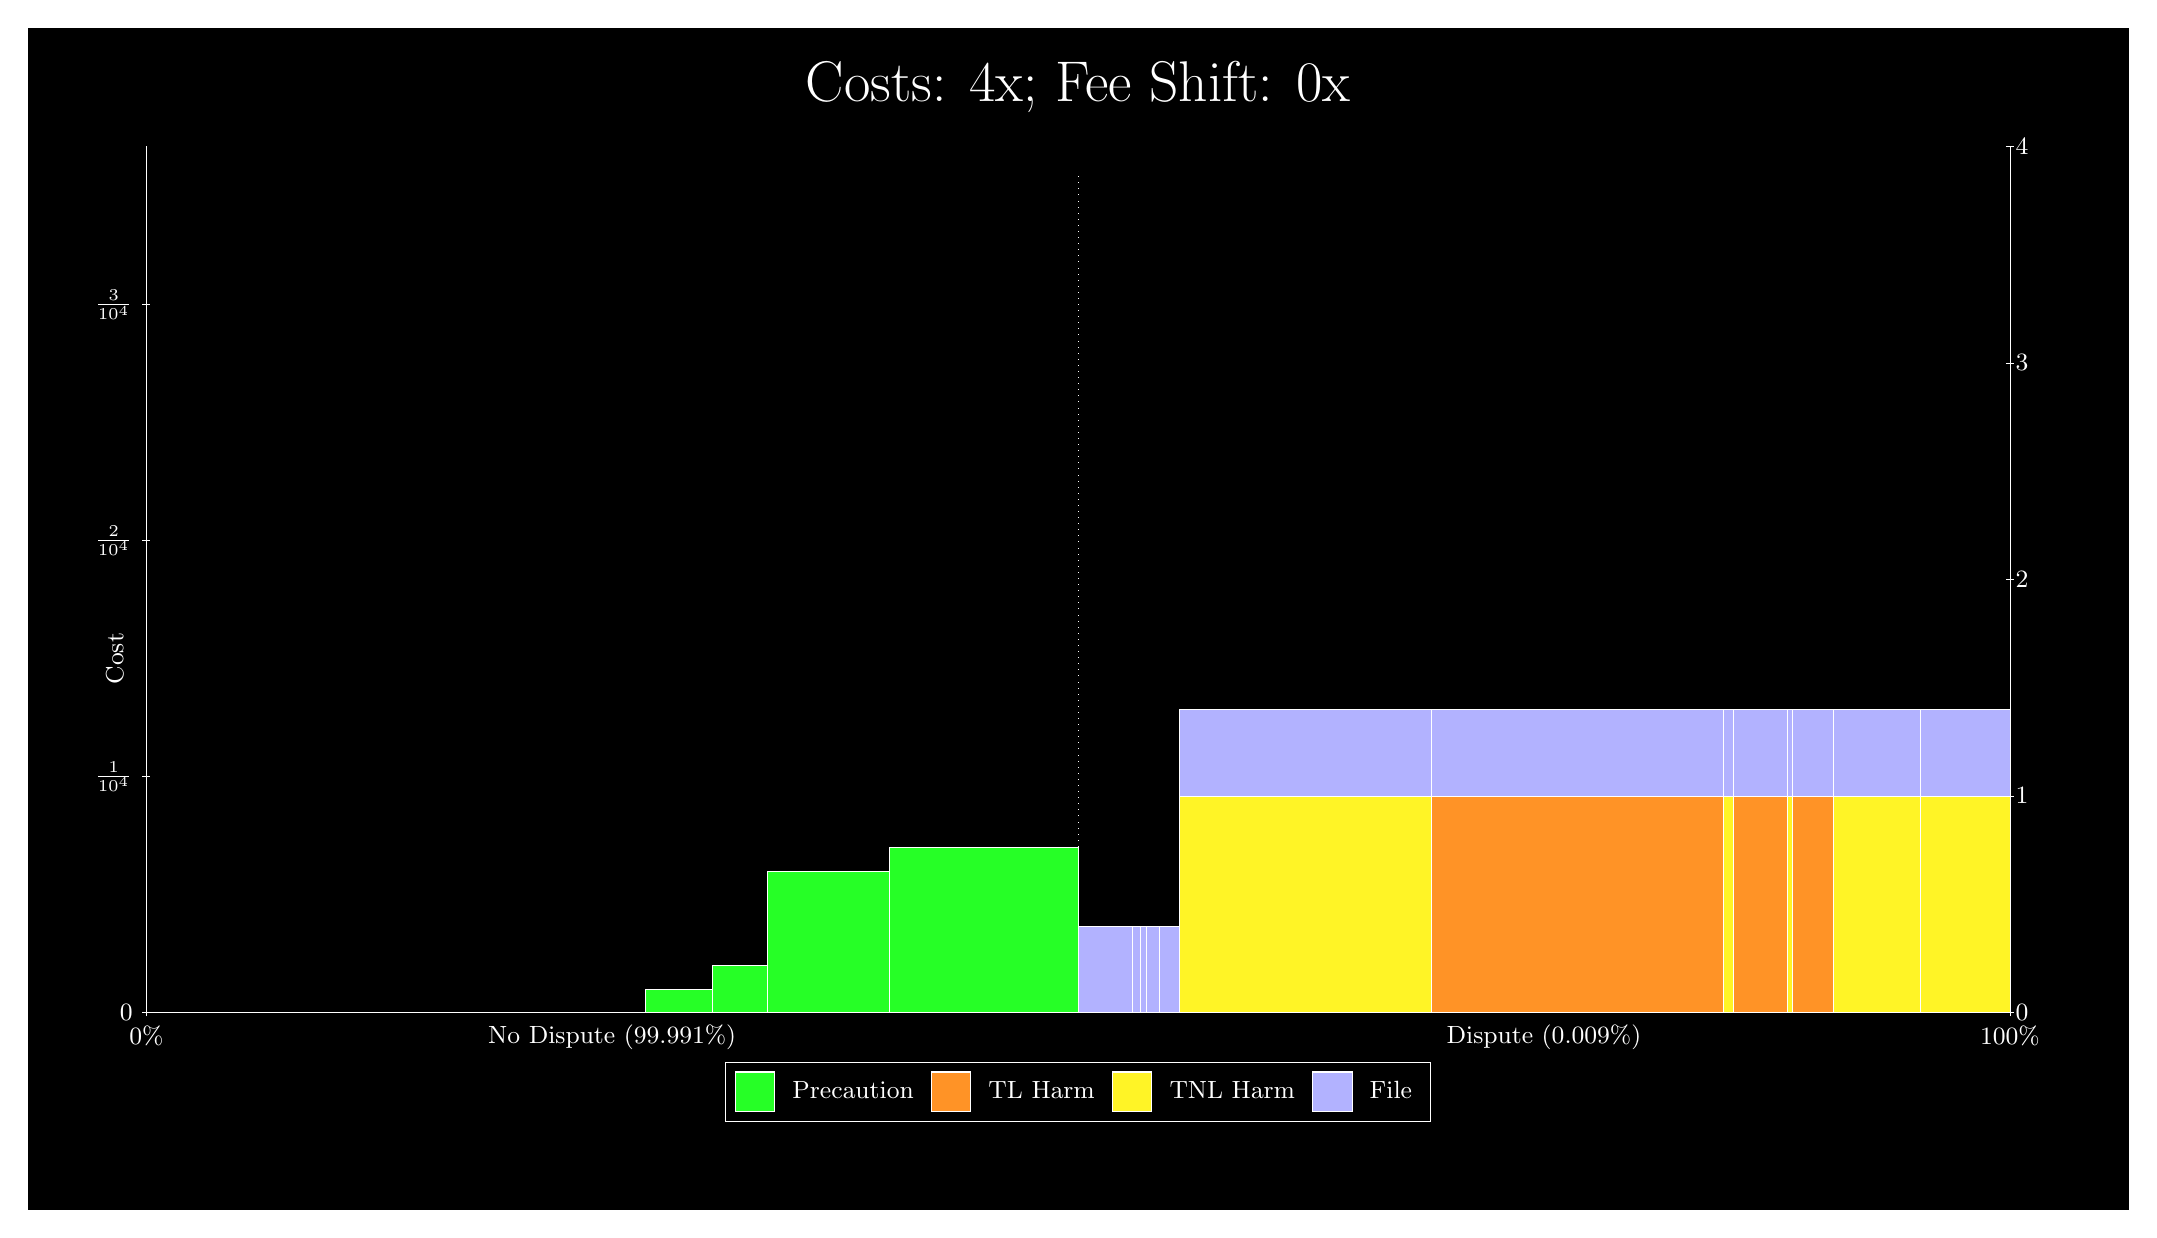
\begin{tikzpicture}
\draw[fill=black] (0,0) rectangle (26.667,15);
\draw[draw=none,text=white] (0,13.5) rectangle (26.667,15) node[midway] {\huge Costs: 4x; Fee Shift: 0x };
\draw[fill=green!85,draw=white,very thin] (7.8418,2.5) rectangle (8.6891,2.7996);
\draw[fill=green!85,draw=white,very thin] (8.6891,2.5) rectangle (9.3888,3.0992);
\draw[fill=green!85,draw=white,very thin] (9.3888,2.5) rectangle (10.936,4.2975);
\draw[fill=green!85,draw=white,very thin] (10.936,2.5) rectangle (13.333,4.5971);
\draw[fill=blue!30,draw=white,very thin] (13.333,2.5) rectangle (14.024,3.6);
\draw[fill=green!85,draw=white,very thin] (14.024,2.5) rectangle (14.117,2.5);
\draw[fill=blue!30,draw=white,very thin] (14.024,2.5) rectangle (14.117,3.6);
\draw[fill=green!85,draw=white,very thin] (14.117,2.5) rectangle (14.193,2.5001);
\draw[fill=blue!30,draw=white,very thin] (14.117,2.5001) rectangle (14.193,3.6001);
\draw[fill=green!85,draw=white,very thin] (14.193,2.5) rectangle (14.361,2.5002);
\draw[fill=blue!30,draw=white,very thin] (14.193,2.5002) rectangle (14.361,3.6002);
\draw[fill=green!85,draw=white,very thin] (14.361,2.5) rectangle (14.622,2.5002);
\draw[fill=blue!30,draw=white,very thin] (14.361,2.5002) rectangle (14.622,3.6002);
\draw[fill=yellow!85,draw=white,very thin] (14.622,2.5) rectangle (17.819,5.25);
\draw[fill=blue!30,draw=white,very thin] (14.622,5.25) rectangle (17.819,6.35);
\draw[fill=orange!85,draw=white,very thin] (17.819,2.5) rectangle (21.532,5.25);
\draw[fill=blue!30,draw=white,very thin] (17.819,5.25) rectangle (21.532,6.35);
\draw[fill=green!85,draw=white,very thin] (21.532,2.5) rectangle (21.658,2.5);
\draw[fill=yellow!85,draw=white,very thin] (21.532,2.5) rectangle (21.658,5.25);
\draw[fill=blue!30,draw=white,very thin] (21.532,5.25) rectangle (21.658,6.35);
\draw[fill=green!85,draw=white,very thin] (21.658,2.5) rectangle (22.345,2.5);
\draw[fill=orange!85,draw=white,very thin] (21.658,2.5) rectangle (22.345,5.25);
\draw[fill=blue!30,draw=white,very thin] (21.658,5.25) rectangle (22.345,6.35);
\draw[fill=green!85,draw=white,very thin] (22.345,2.5) rectangle (22.399,2.5001);
\draw[fill=yellow!85,draw=white,very thin] (22.345,2.5001) rectangle (22.399,5.2501);
\draw[fill=blue!30,draw=white,very thin] (22.345,5.2501) rectangle (22.399,6.3501);
\draw[fill=green!85,draw=white,very thin] (22.399,2.5) rectangle (22.92,2.5001);
\draw[fill=orange!85,draw=white,very thin] (22.399,2.5001) rectangle (22.92,5.2501);
\draw[fill=blue!30,draw=white,very thin] (22.399,5.2501) rectangle (22.92,6.3501);
\draw[fill=green!85,draw=white,very thin] (22.92,2.5) rectangle (24.033,2.5002);
\draw[fill=yellow!85,draw=white,very thin] (22.92,2.5002) rectangle (24.033,5.2502);
\draw[fill=blue!30,draw=white,very thin] (22.92,5.2502) rectangle (24.033,6.3502);
\draw[fill=green!85,draw=white,very thin] (24.033,2.5) rectangle (25.167,2.5002);
\draw[fill=yellow!85,draw=white,very thin] (24.033,2.5002) rectangle (25.167,5.2502);
\draw[fill=blue!30,draw=white,very thin] (24.033,5.2502) rectangle (25.167,6.3502);
\draw[white,very thin] (1.5,2.5) -- (1.5,13.5);
\node[font=\small,rotate=90,text=white, anchor=center] at (1.1, 6.9938) {Cost};
\draw[white,very thin] (1.45,2.5) -- (1.55,2.5);
\node[font=\small,text=white, anchor=east] at (1.45, 2.5) {0};
\draw[white,very thin] (1.45,5.4959) -- (1.55,5.4959);
\node[font=\small,text=white, anchor=east] at (1.45, 5.4959) {$\frac{1}{10^{4}}$};
\draw[white,very thin] (1.45,8.4918) -- (1.55,8.4918);
\node[font=\small,text=white, anchor=east] at (1.45, 8.4918) {$\frac{2}{10^{4}}$};
\draw[white,very thin] (1.45,11.488) -- (1.55,11.488);
\node[font=\small,text=white, anchor=east] at (1.45, 11.488) {$\frac{3}{10^{4}}$};

\draw[white,dotted,very thin] (13.333,2.83) -- (13.333,13.17);
\draw[white,very thin] (25.167,2.5) -- (25.167,13.5);
\draw[white,very thin] (25.117,2.5) -- (25.217,2.5);
\node[font=\small,text=white, anchor=west] at (25.117, 2.5) {0};
\draw[white,very thin] (25.117,5.25) -- (25.217,5.25);
\node[font=\small,text=white, anchor=west] at (25.117, 5.25) {1};
\draw[white,very thin] (25.117,8) -- (25.217,8);
\node[font=\small,text=white, anchor=west] at (25.117, 8) {2};
\draw[white,very thin] (25.117,10.75) -- (25.217,10.75);
\node[font=\small,text=white, anchor=west] at (25.117, 10.75) {3};
\draw[white,very thin] (25.117,13.5) -- (25.217,13.5);
\node[font=\small,text=white, anchor=west] at (25.117, 13.5) {4};

\draw[white,very thin] (1.5,2.5) -- (25.167,2.5);
\draw[white,very thin] (1.5,2.45) -- (1.5,2.55);
\node[font=\small,text=white, anchor=north] at (1.5, 2.45) {0\%};
\draw[white,very thin] (25.167,2.45) -- (25.167,2.55);
\node[font=\small,text=white, anchor=north] at (25.167, 2.45) {100\%};

\node[font=\small,text=white,anchor=south] at (7.4167, 1.9) {No\ Dispute\ (99.991\%)};
\node[font=\small,text=white,anchor=south] at (19.25, 1.9) {Dispute\ (0.009\%)};
\draw (13.3333,2.5) node (B) {};
\begin{scope}[align=center]
\matrix[scale=0.5,draw=white,below=0.5cm of B,nodes={draw},column sep=0.1cm]{
\node[rectangle,draw,minimum width=0.5cm,minimum height=0.5cm,fill=green!85]{}; & \node[draw=none,font=\small,text=white]{Precaution}; &
\node[rectangle,draw,minimum width=0.5cm,minimum height=0.5cm,fill=orange!85]{}; & \node[draw=none,font=\small,text=white]{TL Harm}; &
\node[rectangle,draw,minimum width=0.5cm,minimum height=0.5cm,fill=yellow!85]{}; & \node[draw=none,font=\small,text=white]{TNL Harm}; &
\node[rectangle,draw,minimum width=0.5cm,minimum height=0.5cm,fill=blue!30]{}; & \node[draw=none,font=\small,text=white]{File}; \\\\
};\end{scope}

\end{tikzpicture}
\end{document}